\documentclass[6pt,landscape,a4paper]{article}
\usepackage[utf8]{inputenc}
%\usepackage[ngerman]{babel}
\usepackage[T1]{fontenc}
%\usepackage[LY1,T1]{fontenc}
%\usepackage{frutigernext}
%\usepackage[lf,minionint]{MinionPro}
\usepackage{tikz}
\usetikzlibrary{shapes,positioning,arrows,fit,calc,graphs,graphs.standard}
\usepackage{lipsum}
\usepackage[nosf]{kpfonts}
%\usepackage[t1]{sourcesanspro}
\usepackage{multicol}
\usepackage{wrapfig}
\usepackage[top=1mm,bottom=6mm,left=3mm,right=3mm]{geometry}
\usepackage[framemethod=tikz]{mdframed}
\usepackage{microtype}
\usepackage{pdfpages}
\usepackage{amsmath}
\usepackage[hidelinks]{hyperref}
\usepackage{mathtools}
\usepackage{eso-pic}
\usepackage{tabularx}
\usepackage{bm}
\usepackage{pgfplots}
\let\bar\overline
\usepackage[skip=0pt, indent=0pt]{parskip}
%\include{inhalt/def}
\usepackage{titlesec}
\titlespacing*{\section}{0pt}{0.001\baselineskip}{0.001\baselineskip}
\titlespacing*{\subsubsection}{0pt}{0.2\baselineskip}{0.1\baselineskip}

\begin{document}
%\setlength{\abovedisplayskip}{0pt}
%\setlength{\belowdisplayskip}{0pt}
%\setlength{\abovedisplayshortskip}{0pt}
%\setlength{\belowdisplayshortskip}{0pt}


\footnotesize
\AddToShipoutPictureBG*{
\AtPageLowerLeft{\raisebox{1\height}{\hspace{0.3cm}{Get this signal processing cheat sheet and the rest of the course material from: \url{https://github.com/jvierine/signal_processing_course}}}}%
}
%\small
\begin{multicols*}{5}
\subsubsection*{Frequencies}
Continuous-time:
$\omega$ (rad/s), $f$ (Hz or 1/s), $\omega = 2\pi f$, period: $T=1/f$ (s)\\
\noindent Discrete-time:
$\hat{\omega}$ (rad/sample), $\omega$ (rad/s), $f_s$ sample-rate (sample/s), $\hat{\omega} = \omega/f_s$.
\tikzset{%
    dimen/.style={|-|,>=latex,thin,every rectangle node/.style={fill=white,midway,font=\sffamily}},
}
\begin{tikzpicture}
      \begin{axis}[domain=0:(2*3.14),
          width=7cm,
          height=5cm,
          ticks=none,
          axis lines = center,
          ymax=2,
          ymin=-1.6,
          samples=200,
          legend pos=north east,
          legend style={draw=none},
          xlabel={$t$},
          ylabel={$e^{i\omega t}$},
          legend style={at={(1,1.06)}}]
        \addplot[blue] {cos(2*deg(x))};
        \addplot[red] {sin(2*deg(x))};

        \node at (axis cs:3.14,-1.5) {$\textstyle{T=2\pi/\omega}$};
        \addplot [dimen] plot coordinates {(1.57,-1.1) (4.71,-1.1)};
        \legend{$\mathrm{Re}(e^{i\omega t})=\cos(\omega t))$,$\mathrm{Im}(e^{i\omega t})=\sin(\omega t)$}
      \end{axis}
    \end{tikzpicture}

\subsubsection*{Sampling}
Aliases of a discretized complex sinusoid:
\begin{align*}
 x[n]  = e^{i(\hat{\omega}_0 + 2\pi k) n} = e^{i\hat{\omega}_0 n} 
\end{align*}
Frequency aliases:
\begin{align*}
    \hat{\omega}_k = \hat{\omega}_0 + 2\pi k
\end{align*}
Principal spectrum
\begin{align*}
 -\pi \le \hat{\omega} < \pi 
 \end{align*}
 Dirac comb:
 \begin{align*}
 s(t) &= \textstyle\sum_{k=-\infty}^{\infty}\delta(t-kT_s)  \\
  &= T_s^{-1}\textstyle\sum_{k=-\infty}^{\infty} e^{i \frac{2\pi}{T_s}kt}.
 \end{align*}
 Idealized sampled signal $\omega_s = 2\pi f_s$:
 \begin{align*}
 x_s(t) &= x(t) s(t) \\
\hat{x}_s(\omega)  &= (2\pi)^{-1} \hat{x}(\omega) * \hat{s}(\omega)\\
&= T_s^{-1} \textstyle\sum_{k=-\infty}^{\infty}\hat{x}(\omega + k \omega_s)
 \end{align*}
Nyquist oversampling criterion ($x(t)\in \mathbb{R}$):
\begin{align*}
f_s > 2 f_{\mathrm{max}}
 \end{align*}
Nyquist undersampling criterion ($x(t)\in \mathbb{R}$):
\begin{align*}
&f_{\mathrm{max}}-f_{\mathrm{min}} < f_s/2 \\ 
&k f_s/2 < f_{\mathrm{min}} < (k+1) f_s/2 \\ 
&k f_s/2 < f_{\mathrm{max}} < (k+1) f_s/2 
 \end{align*}
$f_{\mathrm{max}}$, and $f_{\mathrm{min}}$ are the largest and smallest positive frequencies in signal, and $k \in \mathbb{N}_{>0}$ is Nyquist zone.

Nyquist sampling criterion ($x(t)\in \mathbb{C}$):
\begin{align*}
&f_{\mathrm{max}}-f_{\mathrm{min}} < f_s 
 \end{align*}
$f_{\mathrm{max}}$, and $f_{\mathrm{min}}$ are the largest and smallest frequencies in signal (can be negative).
\subsubsection*{Convolution}
\vspace{-0.8em}
\begin{align*}
x_1(t)*x_2(t) &:= \textstyle\int_{-\infty}^{\infty} x_1(\tau) x_2(t-\tau)d\tau \\
x_1[n]*x_2[n] &:= \textstyle\sum_{k=-\infty}^{\infty} x_1[k] x_2[n-k]
\end{align*}
Identity: $x[n]*\delta[n]=x[n]$\\
Commutative: $a[n] * b[n] = b[n] * a[n]$\\
Associative  $(a[n]*b[n]) * c[n] = a[n] * ( b[n] * c[n])$ \\
Distributive: \\
$a[n]*(b[n]+c[n]) = a[n]*b[n] + a[n]*c[n]$   

\subsubsection*{Fourier Series}
Synthesis ($x_N(t) = x_N(t+T)$)
\begin{align*}
x_N(t) = \textstyle\sum_{k=-N}^{N} c_k e^{i \frac{2\pi}{T}kt}
\end{align*}
Analysis ($t_0$ is an arbitrary constant):
\begin{align*}
c_k = T^{-1}\textstyle\int_{t_0}^{t_0+T} x(t)e^{-\frac{2\pi}{T}kt}dt
\end{align*}
Test for periodicity: all frequencies in $\textstyle\sum_k c_k e^{i\omega_k t}$ are commensurable, i.e. $\omega_k / \omega_{\ell} = n/m \in \mathbb{Q}$ with $k,\ell,m,n \in \mathbb{Z}$.
\subsubsection*{Fourier Transform}
Forward
\vspace{-1em}
\begin{align*}
x(t) = \frac{1}{2\pi}\textstyle\int_{-\infty}^{\infty}\hat{x}(\omega)e^{i\hat{\omega}t}d\omega
\end{align*}
Reverse
\vspace{-1em}
\begin{align*}
\hat{x}(\omega)=\textstyle\int_{-\infty}^{\infty} x(t) e^{-i\omega t}dt
\end{align*}
Important transforms:
\begin{align*}
 & x(t)  \xleftrightarrow{\mathcal{F}}  \hat{x}(\omega) \hspace{1.5em}  \delta(t+\tau) \xleftrightarrow{\mathcal{F}}  e^{i\omega \tau}\\
&    e^{i\omega_0 t} \xleftrightarrow{\mathcal{F}}  2\pi \delta(\omega-\omega_0)  \hspace{1em}    x(t-t_0) \xleftrightarrow{\mathcal{F}} e^{-i\omega t_0}\hat{x}(\omega)     \\
&    u\left(t+T/2\right) - u\left(t-T/2\right) \xleftrightarrow{\mathcal{F}} 2\sin(\omega T/2)/\omega\\
&    e^{-\alpha t^2} \xleftrightarrow{\mathcal{F}} \sqrt{\pi/\alpha} e^{-\frac{\omega^2}{4\alpha}} \hspace{1em}    e^{-\beta t} u(t) \xleftrightarrow{\mathcal{F}} 1/(\beta + i\omega)\\
&     x(at) \xleftrightarrow{\mathcal{F}}  |a|^{-1}\hat{x}(\omega/a)  \hspace{1em}   e^{i\omega_0 t}x(t) \xleftrightarrow{\mathcal{F}}  \hat{x}(\omega - \omega_0)  
\end{align*}
Convolution theorem:
\begin{align*}
&x_1(t)*x_2(t) \xleftrightarrow{\mathcal{F}} \hat{x}_1(\omega)\hat{x}_2(\omega) \\
&x_1(t)x_2(t) \xleftrightarrow{\mathcal{F}} (2\pi)^{-1}\hat{x}_1(\omega) * \hat{x}_2(\omega)
\end{align*}
Plancherel's theorem:
\begin{align*}
        \textstyle\int_{-\infty}^{\infty} f(t) g^*(t) dt = \frac{1}{2\pi} \textstyle\int_{-\infty}^{\infty}  \hat{F}(\omega)\hat{G}^*(\omega) d\omega\,\,.
\end{align*}
Parseval's theorem:
\begin{align*}
        \textstyle\int_{-\infty}^{\infty} |x(t)|^2 dt = \frac{1}{2\pi} \textstyle\int_{-\infty}^{\infty} | \hat{x}(\omega)|^2 d\omega
\end{align*}
\subsubsection*{Z-transform}
%The Z-transform is a discrete-time Laplace-transform. It allows algebraic manipulation of polynomials to be used for analysis and design of signals and systems.
Forward:
\vspace{-1em}
\begin{align*}
X(z) = \textstyle\sum_{k=-\infty}^{\infty} x[k] z^{-k}
\end{align*}
Reverse:
\vspace{-1em}
\begin{align*}
    x[n] = \mathcal{Z}^{-1}\{X(z)\} =  \frac{1}{2 \pi i} \textstyle\oint_{C} X(z) z^{n-1} dz
\end{align*}
Infinite impulse response system:
\begin{align*}
        y[n] &= \textstyle\sum_{\ell=1}^{N} a_{\ell} y[n-\ell] + \textstyle\sum_{k=0}^{M} b_k x[n-k]\\
\mathcal{H}(z)&= \frac{\textstyle\sum_{k=0}^{M}b_k z^{-k}}{1-\textstyle\sum_{\ell=1}^{N}a_\ell z^{-\ell}} = \frac{\prod_{k=1}^M(1-\alpha_k z^{-1})}{\prod_{\ell=1}^N(1-\beta_{\ell} z^{-1})}
\end{align*}
Poles: $\beta_{\ell} \in \mathbb{C}$, Zeros: $\alpha_k \in \mathbb{C}$.

\noindent Z-transform pairs:
\begin{align*}
&\mathcal{H}(\hat{\omega})=\left.\mathcal{H}(z)\right|_{z=e^{i\hat{\omega}}} \hspace{1em} a \delta[n-n_0] \xleftrightarrow{\mathcal{Z}} az^{-n_0} \\
& b a^n u[n] \xleftrightarrow{\mathcal{Z}} \frac{b}{1-az^{-1}} \hspace{1em} a[n]*b[n] \xleftrightarrow{\mathcal{Z}} A(z)B(z) 
\end{align*}
Bounded Input Bounded Output stability:
\begin{align*}
\textstyle\sum_{k=-\infty}^{\infty} |h[k]| \le M < \infty
\end{align*}
\subsubsection*{Discrete-time Fourier Transform}
Reverse
\vspace{-1em}
\begin{align*}
x[n]=\frac{1}{2\pi}\textstyle\int_{-\pi}^{\pi}\hat{x}(\hat{\omega})e^{i\hat{\omega}n}d\hat{\omega}
\end{align*}
Forward
\vspace{-1em}
\begin{align*}
\hat{x}(\hat{\omega})=\textstyle\textstyle\sum_{n=-\infty}^{\infty} x[n] e^{-i\hat{\omega} n}
\end{align*}
Important transforms:
\begin{align*}
&x[n]  \xleftrightarrow{\mathcal{F}} \hat{x}(\hat{\omega}) \hspace{1em} a \delta[n-n_0] \xleftrightarrow{\mathcal{F}} a e^{i\hat{\omega}n_0}  \\
&x[n]*y[n] \xleftrightarrow{\mathcal{F}} \hat{x}(\hat{\omega})\hat{y}(\hat{\omega}) \\ &e^{i\hat{\omega}_0 n}x[n] \xleftrightarrow{\mathcal{F}} \hat{x}(\hat{\omega} - \hat{\omega}_0)\\
&\textstyle\sum_{k=-N}^{N} \delta[n-k] \xleftrightarrow{\mathcal{F}} \frac{\sin(\hat{\omega}M/2)}{\sin(\hat{\omega}/2)}
\end{align*}
\subsubsection*{Discrete Fourier Transform}
Forward:
\begin{align*}
\hat{x}[k] = \textstyle\sum_{n=0}^{N-1}x[n]e^{-i\frac{2\pi}{N}kn}
\end{align*}
Reverse:
\vspace{-1em}
\begin{align*}
x[n] = \frac{1}{N}\textstyle\sum_{k=0}^{N-1}\hat{x}[k]e^{i\frac{2\pi}{N}kn}
\end{align*}
$x[n]=x[n+N]$, $\hat{x}[k]=\hat{x}[k+N]$, $k\in \{0,1,2,\cdots,N-1\}$, $n\in \{0,1,2,\cdots,N-1\}$\\
Principal spectrum frequency:
\begin{align*}
&  \hat{\omega}_k = \left\{\begin{array}{cl}
    2\pi k/N & ~  k \le N/2   \\
    2\pi k/N - 2\pi & ~  N/2 < k \le N-1 \\
  \end{array}
  \right.
\end{align*}
\if 0
\begin{align*}
&  f_k = \left\{\begin{array}{cl}
    f_s k/N & ~  k \le N/2   \\
    f_s k/N - f_s & ~  N/2 < k \le N-1 \\
  \end{array}
  \right.
\end{align*}
\fi
Frequency step: \\
$\Delta{\hat{\omega}}=2\pi/N$ or $\Delta f = f_s/N$.

Periodic convolution:
\begin{align*}
  a[n] \circledast b[n] = \textstyle\sum_{k=0}^{N-1} a[k]b[(n-k) \mod N] \,\,.
\end{align*}
Periodic convolution theorem:
\begin{align*}
    a[n] \circledast b[n] \xleftrightarrow{\mathcal{F}} \hat{a}[k]\hat{b}[k]
\end{align*}

DFT matrix $\bm{\hat{x}}=\bm{F}\bm{x}$:
\begin{align*}
&\begin{bmatrix}
                               \phi^{0\cdot0}     & \phi^{0 \cdot 1}         & \cdots & \phi^{0 \cdot (N-1)}     \\
                               \phi^{1\cdot0}     & \phi^{1 \cdot 1}        & \cdots & \phi^{1 \cdot (N-1)}     \\
                               \phi^{2\cdot0}      & \phi^{2 \cdot 2}     & \cdots & \phi^{2 \cdot (N-1)}     \\
                               \vdots             &                      &                       \ddots & \vdots                   \\
                               \phi^{(N-1)\cdot0} & \phi^{(N-1) \cdot 1}  & \cdots & \phi^{(N-1) \cdot (N-1)} \\
                             \end{bmatrix} \,\,.
\end{align*}
here $\phi=e^{-i 2\pi/N}$
\subsubsection*{Ideal discrete-time filters}
Low-pass filter:
\begin{align*}
    \frac{\sin(\hat{\omega}_0 n)}{\pi n}  &\xleftrightarrow{\mathcal{F}}  = u(\hat{\omega}+\hat{\omega}_0)-u(\hat{\omega}-\hat{\omega}_0)
\end{align*}
High-pass:
\begin{align*}
\delta[n] - \frac{\sin(\hat{\omega}_0 n)}{\pi n} &\xleftrightarrow{\mathcal{F}}  1-[u(\hat{\omega}+\omega_0)-u(\hat{\omega}-\omega_0)] 
\end{align*}
Point-frequency:
\begin{align*}
    (2\pi)^{-1} e^{i\hat{\omega}_0 n} &\xleftrightarrow{\mathcal{F}}  \delta(\hat{\omega}-\hat{\omega}_0)
\end{align*}
\subsubsection*{Tapering windows}
Hann window
\begin{align*}
  w[n] =\left\{ \begin{array}{cc}
    \sin^2(\pi n/N) & 0 \le n \le N-1     \\
    0               & \mathrm{otherwise}.
  \end{array}
  \right.
  \label{eq:hann_window_def}
\end{align*}
\subsubsection*{Time-frequency uncertainty}
The width of a function in time domain ($\Delta t$) is inversely proportional to width in frequency domain ($\Delta f$):
\vspace{-0.5em}
\begin{align*}
&\Delta f \Delta t = \gamma  \hspace{3em} x(at) \xleftrightarrow{\mathcal{F}} |a|^{-1}\hat{x}(\omega/a)
\end{align*}
where $\gamma$ is a constant that depends on definition of width. E.g. diffraction limit of an optical system: $\theta \propto \lambda/D$, or frequency resolution of a filter: $\Delta f \propto 1/\Delta t$.
\subsubsection*{Linear Time-Invariant Systems}
Linearity
\begin{align*}
\mathcal{T}\{ c_1 x_1[n] + c_2 x_2[n]\}=c_1\mathcal{T}\{ x_1[n] \} + c_2 \mathcal{T}\{ x_2[n] \}
\end{align*}
Time-invariance
\begin{align*}
\mathcal{D}\{\mathcal{T}\{ x[n] \} = \mathcal{T}\{\mathcal{D}\{ x[n] \} 
\end{align*}
Here $\mathcal{D}$ is time-shift: $\mathcal{D}\{x(t)\}=x(t-\tau)$.

LTI system eigenfunction: 
\begin{align*}
\mathcal{T}\{A e^{i\phi} e^{i\omega t}\}=A' e^{i\phi'}e^{i\omega t}
\end{align*}
Impulse response fully characterizes:
\begin{align*}
&h(t) = \mathcal{T}\{\delta(t)\} \hspace{3em} h[n]  = \mathcal{T}\{\delta[n]\} \\
&y(t) = \mathcal{T}\{x(t)\} = h(t)*x(t) \\
&y[n]  = \mathcal{T}\{x[n]\} = h[n]*x[n]
\end{align*}
Frequency response:
\begin{align*}
  \mathcal{H}(\omega) &= \textstyle\int_{-\infty}^{\infty} h(\tau) e^{-i \omega \tau} d\tau \\
    \mathcal{H}(\hat{\omega}) &= \textstyle\sum_{n=-\infty}^{\infty} h[n] e^{-i \hat{\omega} n} \\
        y(t) = h(t)*x(t) &\xleftrightarrow{\mathcal{F}} \hat{y}(\omega)=\mathcal{H}(\omega)\hat{x}(\omega) \\
     y[n] = h[n]*x[n] &\xleftrightarrow{\mathcal{F}} \hat{y}(\hat{\omega})=\mathcal{H}(\hat{\omega})\hat{x}(\hat{\omega}) 
\end{align*}
Magnitude response: $|\mathcal{H}(\omega)|$, phase response: $\angle \mathcal{H}(\omega)$. Magnitude response often reported in decibel: $10\log_{10}(|\mathcal{H}(\omega)|^2)$,

\subsubsection*{Decibel (dB)}
\begin{tabularx}{\columnwidth}{ll|ll|ll}
dB & linear & dB & linear & dB & linear \\
\hline
7  & 5.01 & 0.5 & 1.12 & 40 & $10^{4}$ \\
6  & 3.98 & 1 & 1.26 & 30 & $10^{3}$ \\
3  & 2.00 &  1.5 & 1.41 & 20 &$10^{2}$  \\
0  & 1.00 & 2 & 1.58 & 10 &  $10$\\
-3  & 0.50 & 5 & 3.16 & -10 & $10^{-1}$ \\
-6  & 0.25 & 8 & 6.31 & -20 & $10^{-2}$ \\
-7  & 0.20 & 9 & 7.94 & -30 & $10^{-3}$ \\
\end{tabularx}
Logarithmic scale of power $P=|z|^2$:
\begin{align*}
 &10 \log_{10}(P/P_{\mathrm{ref}})
 &20 \log_{10}(|z|/P_{\mathrm{ref}})
\end{align*}
Reference power often unity: $P_{\mathrm{ref}}=1$\\
Signal power (dBm): $P_{\mathrm{ref}}=10^{-3}$ W\\
Radar cross-section (dBsm): $P_{\mathrm{ref}}=1$ m$^{2}$\\
Sound intensity ($L_p$): $P_{\mathrm{ref}}=1$ pW/m$^{2}$ 
\subsubsection*{Elementary signals}
Dirac-delta (unit impulse)
\begin{align*}
\textstyle\int_{-\infty}^{\infty} x(t) \delta(t-\tau)d\tau = x(\tau)
\end{align*}
Unit impulse
\begin{align*}
  &\delta[n] = \left\{\begin{array}{cl}
    1 & ~ n = 0   \\
    0 & ~ n \ne 0 \\
  \end{array}
\right.
  \delta(t) = \left\{\begin{array}{cl}
    \rightarrow \infty & ~ t = 0   \\
    0 & ~t \ne 0 \\
  \end{array}
  \right.
\end{align*}
Unit-step (Heaviside-function):
\begin{align*}
&  u[n] = \left\{\begin{array}{cl}
    0 & ~ n < 0   \\
    1 & ~ n \ge 0 \\
  \end{array}
  \right.
&  u(t) = \left\{\begin{array}{cl}
    0 & ~ t < 0   \\
    1 & ~ t \ge 0 \\
  \end{array}
  \right. 
\end{align*}

\subsubsection*{Misc}
L'H\^opital:
\vspace{-2em}
\begin{align*}
\lim_{n\rightarrow c}\frac{f(n)}{g(n)}=\lim_{n\rightarrow c}\frac{f'(n)}{g'(n)}
\end{align*}
\vspace{-1em}
Geometric series:
\begin{align*}
\textstyle\sum_{k=0}^{n} r^k = \frac{1-r^{n+1}}{1-r}
\end{align*}
%\subsubsection*{Python}
\subsubsection*{Complex number}
\begin{align*}
i &= \sqrt{-1} \hspace{2em} z = x+iy \hspace{2em} z^* = x-iy  \\
|z|^2 &= z z^* \hspace{2em} \angle z = \tan^{-1}(y/x) \hspace{2em} z=|z| e^{i\angle z} \\
e^0 &= 1 \hspace{2em} e^{\pm i\pi} = -1 \hspace{2em} e^{\pm i\pi/2} = \pm i
\end{align*}
Euler's formula:
\vspace{-0.5em}
\begin{align*}
e^{i\theta} &= \cos(\theta) + i\sin(\theta)\\
\cos(\theta) &= 2^{-1}(e^{i\theta}+e^{-i\theta})\\
\sin(\theta) &= (2i)^{-1}(e^{i\theta}-e^{-i\theta})\\
\mathrm{Re}\{z\} &= 2^{-1}(z+z^*)\\
\mathrm{Im}\{z\} &= (2i)^{-1}(z-z^*)
\end{align*}
N$^{\mathrm{th}}$ root of unity ($z^N=1$):
\vspace{-0.7em}
\begin{align*}
z=e^{i2\pi k/N}~~~ k \in \{0,1,2,\cdots,N-1\}
\end{align*}
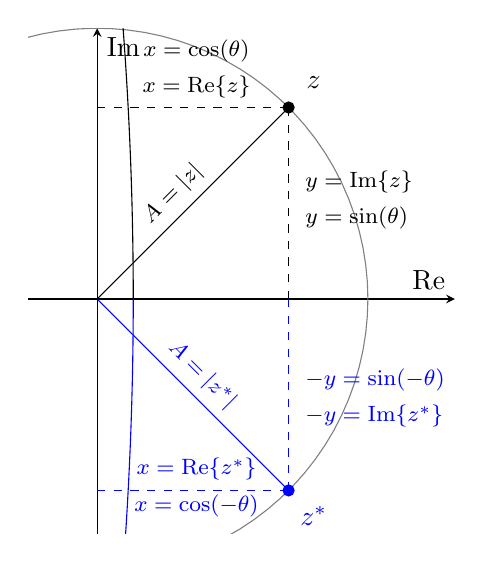
\begin{tikzpicture}
      \begin{axis}[axis equal, ymin=-1.3,xmin=-0.2,ymax=1.5,xmax=1.8,  ticks=none,
          xlabel=$\mathrm{Re}$,
          ylabel=$\mathrm{Im}$, axis lines = center, width=7cm, height=8cm]

        \addplot [gray,domain=0:2*pi,samples=100]({1.5*cos(deg(x))},{1.5*sin(deg(x))});

        \addplot [black, mark = *] coordinates {( {1.5*cos(45)}, {1.5*sin(45)} )} {};
        \addplot [blue, mark = *] coordinates {( {1.5*cos(-45)}, {1.5*sin(-45)} )} {};        
        %   \addplot [black, mark = *] coordinates {( {1.5*cos(-60)}, {1.5*sin(-60)} )} {};   

        \addplot [black] coordinates { (0,0) ( {1.5*cos(45)}, {1.5*sin(45)} ) };

        \addplot [blue] coordinates { (0,0) ( {1.5*cos(-45)}, {1.5*sin(-45)} ) };

        \addplot [dashed,black] coordinates { ({1.5*cos(45)},0) ( {1.5*cos(45)}, {1.5*sin(45)} ) };

        \addplot [dashed,blue] coordinates { ({1.5*cos(45)},0) ( {1.5*cos(45)}, {1.5*sin(-45)} ) };

        \addplot [dashed,black] coordinates { (0,{1.5*sin(45)}) ( {1.5*cos(45)}, {1.5*sin(45)} ) };

        \addplot [dashed,blue] coordinates { (0,{1.5*sin(-45)}) ( {1.5*cos(45)}, {1.5*sin(-45)} ) };

        \draw[draw=black] (axis cs:0.2,0.00) arc [radius={transformdirectionx(0.2)},start angle=0,end angle=45]
        node[midway,right,inner sep=3pt,font={\footnotesize}]{$\theta=\angle z$};

        \draw[draw=blue] (axis cs:0.2,0.00) arc [radius={transformdirectionx(0.2)},start angle=0,end angle=-45]
        node[midway,right,inner sep=3pt,font={\footnotesize}]{{\color{blue}$-\theta=\angle z^*$}};

        \node at (axis cs:0.55,1.06) [above, font={\footnotesize}]{$x=\mathrm{Re}\{z\}$};
        \node at (axis cs:0.55,1.26) [above, font={\footnotesize}]{$x=\cos(\theta)$};        
        \node at (axis cs:0.55,-1.06) [above, font={\footnotesize}]{{\color{blue}$x=\mathrm{Re}\{z^*\}$}};
        \node at (axis cs:0.55,-1.26) [above, font={\footnotesize}]{{\color{blue}$x=\cos(-\theta)$}};                

        \node at (axis cs:1.1,0.65) [right, font={\footnotesize}]{$y=\mathrm{Im}\{z\}$};
        \node at (axis cs:1.1,0.45) [right, font={\footnotesize}]{$y=\sin(\theta)$};        
        \node at (axis cs:1.1,-0.65) [right, color=blue, font={\footnotesize}]{$-y=\mathrm{Im}\{z^*\}$};
        \node at (axis cs:1.1,-0.45) [right, color=blue, font={\footnotesize}]{$-y=\sin(-\theta)$};        

        \node at (axis cs:1.2,1.2) {$z$};
        \node at (axis cs:1.2,-1.2) {{\color{blue}$z^*$}};        

        \node at (axis cs:0.5,0.5) [above,rotate=45,font={\footnotesize}]{$A=|z|$};
        \node at (axis cs:0.5,-0.5) [above,rotate=-45,font={\footnotesize}]{{\color{blue}$A=|z^*|$}};        
      \end{axis}
    \end{tikzpicture}
%\subsubsection*{Complex sinusoid}

\subsubsection*{Fast Fourier Transform}
The most important signal processing algorithm. Efficient Discrete Fourier Transform implementation. $\mathcal{O}(N \log N)$ computational complexity.

Can be used for: convolution, deconvolution, differential equation solving, signal compression, spectral analysis, modulation and demodulation, interpolation and resampling, filtering, matrix diagonalization, calculating polynomial coefficients, estimating a Fourier transform or a discrete-time Fourier transform, channelizing signals (polyphase filterbank), etc.
\\
Implementations

Python: \verb|numpy.fft|, \verb|scipy.fft|, \verb|pyfftw|; C, Fortran, C++: FFTW, Intel MKL; vDSP.FFT; CUDA: CuFFT


\subsubsection*{Add your own notes here...}
\end{multicols*}
\end{document}
